%!TEX root = ../template.tex
%%%%%%%%%%%%%%%%%%%%%%%%%%%%%%%%%%%%%%%%%%%%%%%%%%%%%%%%%%%%%%%%%%%%
%% appendix1.tex
%% NOVA thesis document file
%%
%% Chapter with example of appendix with a short dummy text
%%%%%%%%%%%%%%%%%%%%%%%%%%%%%%%%%%%%%%%%%%%%%%%%%%%%%%%%%%%%%%%%%%%%

\typeout{NT FILE appendix1.tex}%

\chapter{Appendix}
\label{app:intro}



\section{Comment Configuration}
\label{app:comment}


\subsection{Comment Configuration Example 1}

\begin{figure}[htbp]
	\centering
	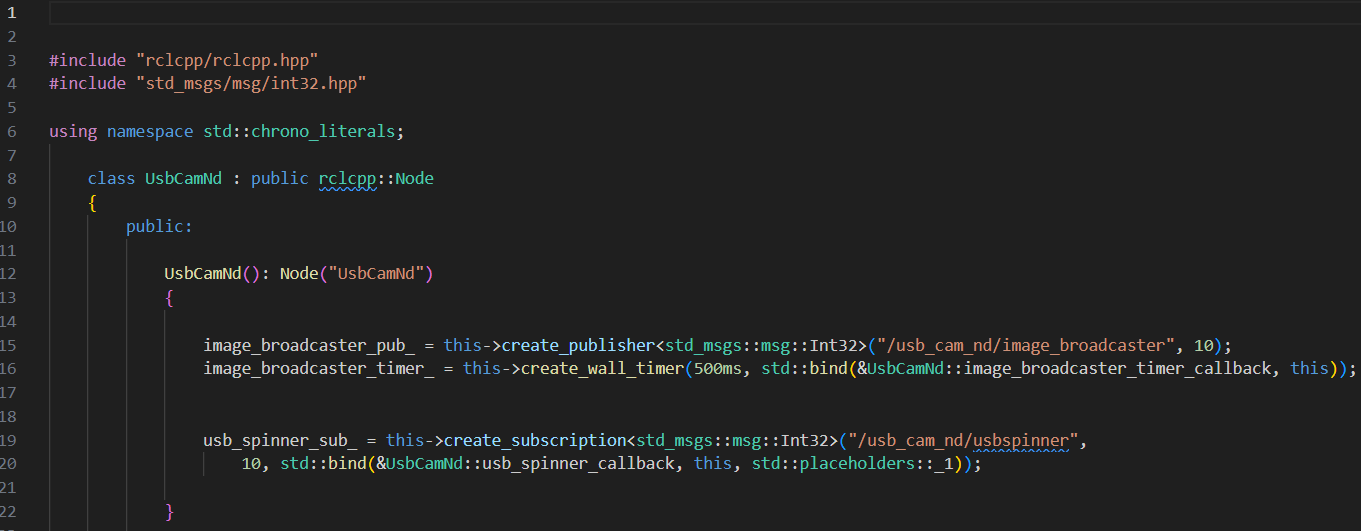
\includegraphics[width=\textwidth]{nocomment_example1.png}
	\caption{Example of generated code without comments}
	\label{figapp:nocomment_example1}
\end{figure}

When code comments are toggled on, the code from Figure~\ref{figapp:nocomment_example1} becomes the code from Figure~\ref{figapp:comment_example1}

\begin{figure}[htbp]
	\centering
	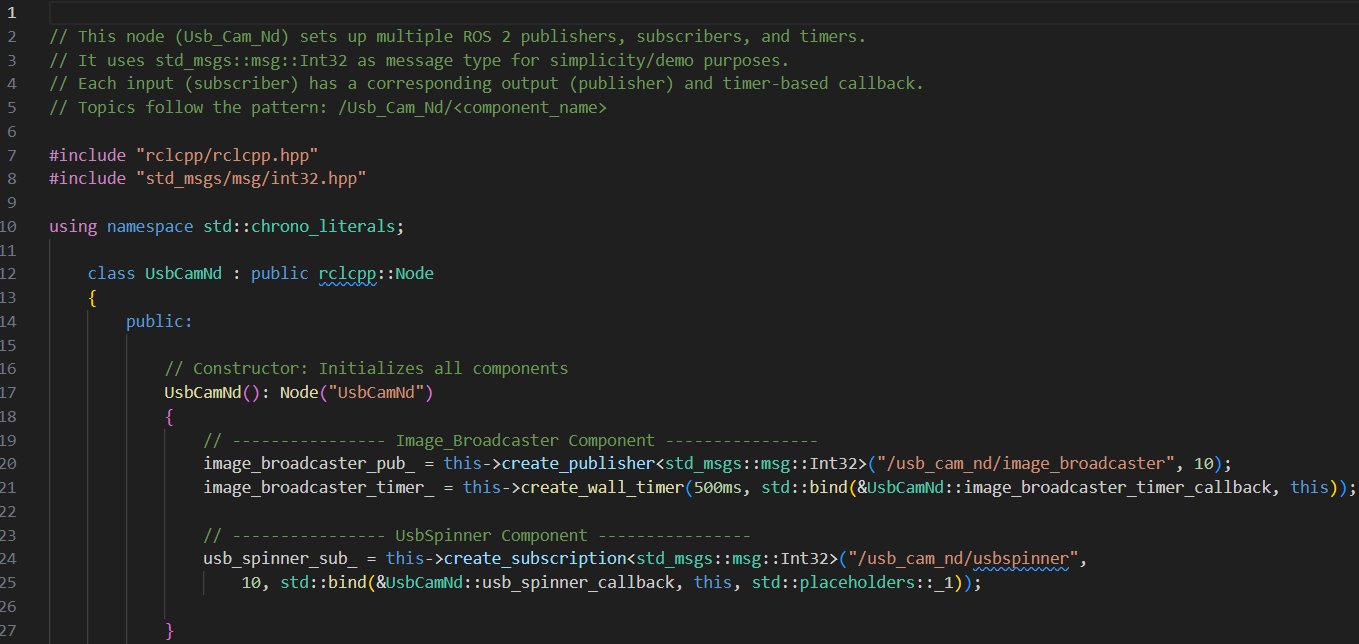
\includegraphics[width=\textwidth]{comment_example1.png}
	\caption{Example of generated code with comments}
	\label{figapp:comment_example1}
\end{figure}

\section{Integration and Regression Tests}
\label{app:int_and_reg_tests}


\bgroup
\rowcolors{1}{}{GhostWhite}
\begin{xltabular}{\textwidth}{X X X}
	\caption{Feature dependency table}
	\label{tab:app_int_and_reg_tests}\\
	\toprule
	\rowcolor{Gainsboro}%
	Feature & Depends On & Notes \\
	\midrule
	Identifiers & – & Core to code structure \\
	Comments & Identifiers & Cheap to implement early \\
	Traceability & Identifiers, Comments & Hard to retrofit later \\
	Report & Traceability & Uses trace data \\
	Standard\par Compliance & Report, Traceability & Enforce compliance early \\
	Dead Code\par Elimination & Traceability, Report & Needs stable generation logic \\
	Memory\par Optimization & Dead Code Elim, Traceability & Impacts data structures directly \\
	Node Interface & Memory Optimization & Enables \gls{ROS} decoupling \\
	Legacy Code\par Integration & Node Interface & Most architecture-dependent \\
	\bottomrule
\end{xltabular}










